\chapter{Aesthetic ideals in programming practices}

The first step in our study of aesthetics in source code aims at identifying the aesthetic ideals that programmers ascribe to source code; that is, the qualifiers and semantic fields that they refer to when discussing program texts. To that end, we first start by clarifying whom we refer to by the term \emph{programmers}, which reveals a multiplicity of practices and purposes, from \emph{ad hoc}, one-line solutions, to printed code and massively-distributed codebases.

We then turn to the kinds of beauty that these programmers aspire to. After expliciting our methodology of discourse analysis, we engage in a review of the various kinds of publications and writings that programmers write, read and refer to when it comes to qualifying their practice. From this will result a clust of adjectives—e.g. \emph{clean}, \emph{simple}, \emph{smelly}—which we argue are used in an aesthetic sense. These will provide a useful framework to inspect, in subsequent chapters, their formal manifestations as typed-out tokens.

From these, we can then move to a description of which aesthetic fields are being referenced by programmers on a broader level, and consider how multiple kinds of beauties, from literary, to architectural and mathematical conceptions of beauty can overlap and be referred to by the same concrete medium.

Finally, we focus our attention on one of the points of overlap in these different references: the importance of function, craft and knowledge in the disposition and representation of code. We will show how this particular way of working  plays a central role in an aesthetic approach to source code and results from the specificity of code as a cognitive material, a specificity we will inquire further in the next chapter.

\section{The practice of programmers}

The history of software development is that of a specific, reserved practice which was born in the aftermath of the second world war, which trickled down to broader and broader audiences at the eve of the twenty-first century. Through this development, multiple ways of doing, approaches and applications have been involved in producing software, resulting in different communities and types of programming. Each of these focus on the description of specific instructions to the computer, but do so with specific characteristics. To this end, we take a socio-historical stance on the field of programming, highlighting how diverse practices emerge at different moments in time, and how they are connected to contemporary technical and economic organizations.

Even though such types of reading and writing source code often overlap with one another, this section will highlight a diversity of more or less loose ways in which code is being written, notably in terms of references—what do they consider good?—, purposes—what do they write for?—and examples—how does their code look like?. First, we take a look at the software industry, to identify professional \emph{software developers}, the large code bases they work on and the specific organizational practices within which they write it. They are responsible for the majority of source code written today, and do so in a professional and productive context, where maintainability, testability and reliability are the main concerns. Then, we turn to a parallel practice, one that is often exhibited by software developers, as they also take on the stance of \emph{hackers}. Disambiguating the term reveals a set of practices where curiosity, cleverness, and idiosyncracy are central, finding unexpected solutions to complex problems, sometimes within artificial constraints. Finally, we look at \emph{scientists} and \emph{poets}. On one end, \emph{scientists} embody a rather academic approach,  focusing on abstract concepts such as simplicity, minimalism and elegance; they are often focused on theoretical issues, such as implementation of algorithms and mathematical models, as well as programming language design. On the other end, \emph{poets} read and write code first and foremost for its textual and semantic qualities, publishing code poems online and in print, and engaging deeply with the range of metaphors allowed by a dynamic linguistic medium such as code.

While this overview encompasses most of the programming practices, we leave aside some approaches to code, mainly because they do not directly engage with the representation of source code as a textual matter. More and more, end-user applications provide the possibility to program in more or less rudimentary ways, something referred to as the "low-code" approach\cite{oreilly_editorial_team_low-code_2021}, and thus contributing to the blurring of boundaries between programmers and non-programmers\footnote{For instance, Microsoft's Visual Basic for Applications, Ableton's Max For Live, MIT's Scrath or McNeel's Grasshopper are all programming frameworks which are not covered within the scope of this study. In the case of VBA and similar office-based high-level programming, it is because such a practice is a highly personal and \emph{ad hoc} one, and therefore is less available for study.}.

\subsection{Software developers}

\subsubsection{From local hardware to distributed software}

As Niklaus Wirth puts it, \emph{the history of software is the history of growth in complexity}\cite{wirth_brief_2008}, while paradoxically, lowering the barrier to entry. As computers' technical abilities in memory managment and processing power increased year on year since the 1950s, the nature of writing instructions shifted accordingly.

In his history of the software industry, Martin Campbell-Kelly traces the development of a discipline through both an economic and a technological lens, and he identifies three consecutive waves in the production of software\cite{campbell-kelly_airline_2003}. During the first period, as soon as the 1950s, and continuing throughout the 1960s, software developers were contractors hired to engage directly with a specific computing machine. These computing, mainframes, were large, expensive, and rigid machines, requiring hardware-specific knowledge of the Assembler instruction set specific to each one, since they didn't feature an operating system which could facilitate some of the more basic memory allocation and input/output functions, and thus interoperable program-writing\footnote{One of the first operating systems, MIT's Tape Director, would be only developped in 1956\cite{ross_personal_1986}}. Two distinct groups of people were involved in the operationalization of such machine: electrical engineers, tasked with designing hardware, and programmers, tasked with implementing the software. While the former historically received the most attention\cite{ross_personal_1986}, the latter was mostly composed of women and, as such, not considered essential in the process\cite{light_when_1999}. At this point, then, programming is closely tied to hardware.

The second period in software development starts in the 1960s, as hardware started to switch from vacuum tubes to transistors and from magnetic core memory to semiconductor memory, making them faster and more capable to handle complex operations.  On the software side, the development of several programming languages, such as FORTRAN, LISP and COBOL, started to address the double issue of portability—having a program run unmodified on different machines with different instruction sets—and expressivity—allowing programmers to use high-level, English-like syntax, rather than assembler instruction codes. By then, programmers are no longer theoretically tied to a specific machine, and therefore acquire a certain autonomy, a recognition which culminates in the naming of the field of \emph{software engineering} in 1968 at a NATO conference\footnote{source?}.

The third and final phase that Campbell-Kelly identifies is that of mass-market production: following the advent of the UNIX family of operating systems, the distribution of the C programming language, the wide availability of C compilers, and the appearance of personal computers such as the Commodore 64, Altair and Apple II, software could be effectively entirely decoupled from hardware\footnote{For a more detailed account of the personal computer revolution, see: Cerruzzi, P., A History of Modern Computing\cite{ceruzzi_history_2003}}. And yet, software immediately enters a crisis, due to software development projects running over time and budget, being unreliable in production and unmaintainable in the long-run. What this highlighted is that the creation of software was no longer a corollary to the design of hardware, and that it would become the main focus of computing as a whole\cite{ceruzzi_history_2003}, and that it should therefore be addressed as such. It is at this time that discussions around best practices in writing source code started to emerge, once the activity of the programmer was no longer restricted to \emph{tricks by means of which he contrived to squeeze the impossible into the constraints of his equipment}\cite{dijkstra_humble_2007}.

This need for a more formal approach to the actual process of programming found one of its most important manifestations in Edsger Djikstra's \emph{Notes on Structured Programming}\cite{dijkstra_chapter_1972}. In it, he argues for moving away from programming as a craft, and towards programming as an organized discipline, with its methodologies and systematization of program construction. Despite its laconic section titles\footnote{See, for instance, Chapter 1: "\emph{On our inability to do much}"}, Djikstra nonetheless contributed to establish a more rigorous typology of the constructs required for reliable, provable programs—based on fundamentals such as sequence, selection, iteration and recursion—, and aimed at the formalization of the practice. Along with other developments (such as Hoare's contribution on proper data structuring\cite{hoare_chapter_1972}, or the rise of object-oriented programming) programming would solidify its foundations as a profession:

\begin{quote}
    We knew how the nonprofessional programmer could write in an afternoon a three-page program that was supposed to satisfy his needs, but how would the professional programmer design a thirty-page program in such a way that he could really justify his design? What intellectual discipline would be needed? What properties could such a professional programmer demand with justification from his programming language, from the formal tool he had to work with? \cite{dijkstra_ew_programming_1977}
\end{quote}

As a result of such interrogations comes an industry-wide search for solutions to the intractable problem of programming: that it is \emph{a technique to manage information which in turn produces information}. To address such a conundrum, a variety of tools, formal methods and management processes enter the market; they aim at acting as a \emph{silver bullet}\cite{brooks_mythical_1975}, addressing the cascade of potential risks\footnote{See \url{https://catless.ncl.ac.uk/Risks/} for such risks} which emerge from large software applications. However, this growth in complexity is also accompanied by a diversification of complexity: as computers become more widely available, and as higher-level programming languages provide more flexibility in their expressive abilities, software engineering is being applied to a variety of domains, each of which might need a specific solution, rather than a generic process. Confronted with this diversity of applications, business literature on software practices flourishes\footnote{See Jackson, Principles of Program Design, or Martin, Clean Code, among others.}, acknowledging that the complexity of software should be tackled at its bottleneck: the reading and writing of source code.

The most recent step in the history of software developers is the popularization of the Internet and of the World Wide Web. Even though the former had existed under as ArpaNet since 1969, the network was only standardized in 1982 and access to it was provided commercially in 1989. Built on top of the Internet, the latter popularized global information exchange, including technical resources to read and write code. Software could now be written by remote individual written on \emph{cloud computing}  platforms, shared through public repositories and deployed via containers with a lower barrier to entry than at the time of source code printed in magazines, of overnight batch processing and of non-time-sharing systems.

\vspace*{1\baselineskip}

These software developers have written some of the largest codebases to this date, mainly because this type of activity represents the largest fraction of programmers. Due to its close ties to commercial distributors, however, source code written in this context often falls under the umbrella of proprietary software, thus made unvailable to the public. Some examples that we include in our corpus are either professional codebases that have been leaked\footnote{Such as the Microsoft Windows XP source code\cite{warren_windows_2020}.}, open-source projects that have come out of business environments, such as Soundcloud's Prometheus, Google's TensorFlow or Facebook's React, or large-scale open-source projects which nonetheless adhere to structured programming guidelines, such as Donald Knuth's TeX typesetting system or the Linux Foundation's Linux kernel.

\subsubsection{Features of the field}

The features of these codebases provide the backdrop to, and start to hint at, the qualities that software developers have come to ascribe to their object of practice. First, the program texts they write are large, much larger than any other codebase included in this study, they often feature multiple programming languages and are highly structured and standardized: each file follows a pre-established convention in programming style, which favors an authoring by multiple programmers without any obvious trace to a single individual authorship. These program texts stand the closest to a programming equivalent of engineering, with its formalisms, standards and usability. From this perspective, the IEEE's Software Engineering Body of Knoweldge (SWEBOK) provides a good starting point to survey the specificities of software developers as source code writers and readers\cite{bourque_swebok_2014}; the main features of which include the definition of requirements, design, construction testing and maintenance.

Software requirements are the acknowledgement of the importance of the \emph{problem domain}, the domain to which the software takes its inputs from, and to which it applies its outputs. For instance, software written for a calculator has arithmetic as its problem domain; software written for a learning management system has students, faculty, education and courses as its problem domain; software written a banking institution has financial transactions, savings accounts, fraud prevention and credit lines as its problem domain. Requirements in software development aim at formalizing as best as possible the elements that must be used by the software in order to perform a successful computation, and an adequate formalization is a fundamental requirement for a successful software application.

Following the identification and codification of requirements, software design relates to the overall organization of the software components, considered not in their textual implementation, but in their conceptual agency. Usually represented through diagrams or modelling languages, it is concerned with \emph{understanding how a system should be
organized and designing the overall structure of that system}\cite{sommerville_software_2010}. Of particular interest is the relationship that is established between software development and architecture. Considered a creative process rather than a strictly rational one, due to the important role of the contexts in which the software will exist (including the problem domain)\cite{sommerville_software_2010}, software architecture is considered essential from a top-down perspective, laying down an abstract blueprint for the implementation of a system, as well as form a bottom-up one, representing how the different components of an existing system interact. This apparent contradiction, and the role of architecture in the creative aspects of software development, will be further explored in chapter 2.

Software construction relates to the actual writing of software, and how to do so in the most reliable way possible. The SWEBOK emphasizes first and foremost the need to minimize complexity\footnote{Following C. Anthony Hoare's assessment in his Turing Award Lecture that \emph{"there are two ways of constructing a software design: one way is to make it so simple that there are obviously no deficiencies, and the other way is to make it so complicated that there are no obvious deficiencies."}}, in anticipation of likely changes and possible reuse by other software systems. Here, the emphasis on engineering is particularly salient: while most would refer to the creation of software as \emph{writing} software, the IEEE document refers to it as \emph{constructing} software\footnote{The term software construction refers to the detailed creation of working software through a combination of coding, verification, unit testing, integration testing, and debugging.\cite{bourque_swebok_2014}.}. Coding is only assessed as a practical consideration, one which should not take up the most attention, if the requirements, design and testing steps are satisfyingly implemented. Conversely, a whole field of business litterature\cite{martin_clean_2008,hendrickson_software_2002,fowler_refactoring_1999,mcconnell_code_2004} has focused specifically on the process of writing code, starting from the assumption that:

\begin{quote}
    We will never be rid of code, because code represents the details of the requirements. At some level those details cannot be ignored or abstracted; they have to be specified. And specifying requirements in such details that a machine can execute them is \emph{programming}.\cite{martin_clean_2008}
\end{quote}

As we see, the tension identified by Djikstra some thirty years before between craft and discipline is still alive and well at the beginning of the twenty-first century, even though the focus on code still relates to the need for reliability and maintainability in a maturing industry.

Software maintenance, finally, relates not to the planning or writing of software, but to its reading. Software is notoriously filled with bugs\footnote{McConnell estimates that the industry average is about 15 - 50 errors per 1000 lines of delivered code.\cite{mcconnell_code_2004}.} and can, at the same time, be easily fixed while already being in a production environment through software update releases. This means that the lifecycle of a software doesn't stop when then first version is written, but rather when it does not run anymore, and this implies that the nature of software allows for it to be edited across time and space, by other programmers which might not have access to the original group of implementers: consequently, software should be first and foremost understandable—SWEBOK lists the first feature of coding as being \emph{techniques for creating understandable source code}\cite{bourque_swebok_2014}. This requirement ties back to one of the main problems of software, which is its notorious cognitive complexity, one that remains at any stage of its development.

\vspace*{1\baselineskip}

What does this look like in practice, then? Ideals of clarity, reusability and reliability—and their opposites—can be found in some of the available code bases of professional software. The paradox to be noted here is that, even though software developers write the most code, it is the least accessible online and, as such, the following excerpts are covering the range of commercial software (Microsoft Windows), licensed and publicly available software (Kirby), and an open-source software (Prometheus).

The first excerpts come from the source code for Microsoft Windows 2000, which was made public in 2004. The program text contains  28,655 files, the largest of our  corpus, by multiple orders of magnitude, with 13,468,327 combined lines and including more than 10 different file extensions. Taking a closer look at some of these files allow us to identify some of the specific features of code written by software developers, and how they specifically relate to architectural choices, collaborative writing and verbosity.

First, the most striking visual feature of the code is its sheer size. Representing such a versatile and low-level system such as an operating system manifest themselves in files that are often above 2000 lines of code. In order to allow abstraction techniques at a higher-level for the end-developer, the operating system needs to do a significant amount of "grunt" work, relating directly to the concrete reality of the hardware platform which needs to be operated. For instance, the initialization of strings of text for the namespaces (a technique directly related to the compartmentalization) is necessary, repetitive work which can be represented using a rhythmic visual pattern, such as in \lstinline{cmdatini.c}:

\begin{lstlisting}[language=C, basicstyle=\tiny]
  {
    ULONG i;

    RtlInitUnicodeString( &CmRegistryRootName,
                          CmpRegistryRootString );

    RtlInitUnicodeString( &CmRegistryMachineName,
                          CmpRegistryMachineString );

    RtlInitUnicodeString( &CmRegistryMachineHardwareName,
                          CmpRegistryMachineHardwareString );

    RtlInitUnicodeString( &CmRegistryMachineHardwareDescriptionName,
                          CmpRegistryMachineHardwareDescriptionString );

    RtlInitUnicodeString( &CmRegistryMachineHardwareDescriptionSystemName,
                          CmpRegistryMachineHardwareDescriptionSystemString );

    RtlInitUnicodeString( &CmRegistryMachineHardwareDeviceMapName,
                          CmpRegistryMachineHardwareDeviceMapString );

    RtlInitUnicodeString( &CmRegistryMachineHardwareResourceMapName,
                          CmpRegistryMachineHardwareResourceMapString );

    RtlInitUnicodeString( &CmRegistryMachineHardwareOwnerMapName,
                          CmpRegistryMachineHardwareOwnerMapString );

    RtlInitUnicodeString( &CmRegistryMachineSystemName,
                          CmpRegistryMachineSystemString );

    RtlInitUnicodeString( &CmRegistryMachineSystemCurrentControlSet,
                          CmpRegistryMachineSystemCurrentControlSetString);

    RtlInitUnicodeString( &CmRegistryUserName,
                          CmpRegistryUserString );

    RtlInitUnicodeString( &CmRegistrySystemCloneName,
                          CmpRegistrySystemCloneString );

    RtlInitUnicodeString( &CmpSystemFileName,
                          CmpRegistrySystemFileNameString );

    RtlInitUnicodeString( &CmRegistryMachineSystemCurrentControlSetEnumName,
                          CmpRegistryMachineSystemCurrentControlSetEnumString);

    RtlInitUnicodeString( &CmRegistryMachineSystemCurrentControlSetEnumRootName,
                          CmpRegistryMachineSystemCurrentControlSetEnumRootString);

    RtlInitUnicodeString( &CmRegistryMachineSystemCurrentControlSetServices,
                          CmpRegistryMachineSystemCurrentControlSetServicesString);

    RtlInitUnicodeString( &CmRegistryMachineSystemCurrentControlSetHardwareProfilesCurrent,
                          CmpRegistryMachineSystemCurrentControlSetHardwareProfilesCurrentString);

    RtlInitUnicodeString( &CmRegistryMachineSystemCurrentControlSetControlClass,
                          CmpRegistryMachineSystemCurrentControlSetControlClassString);

    RtlInitUnicodeString( &CmRegistryMachineSystemCurrentControlSetControlSafeBoot,
                          CmpRegistryMachineSystemCurrentControlSetControlSafeBootString);

    RtlInitUnicodeString( &CmRegistryMachineSystemCurrentControlSetControlSessionManagerMemoryManagement,
                          CmpRegistryMachineSystemCurrentControlSetControlSessionManagerMemoryManagementString);

    RtlInitUnicodeString( &CmRegistryMachineSystemCurrentControlSetControlBootLog,
                          CmpRegistryMachineSystemCurrentControlSetControlBootLogString);

    RtlInitUnicodeString( &CmRegistryMachineSystemCurrentControlSetServicesEventLog,
                          CmpRegistryMachineSystemCurrentControlSetServicesEventLogString);

    RtlInitUnicodeString( &CmSymbolicLinkValueName,
                          CmpSymbolicLinkValueName);

#ifdef _WANT_MACHINE_IDENTIFICATION
    RtlInitUnicodeString( &CmRegistryMachineSystemCurrentControlSetControlBiosInfo,
                          CmpRegistryMachineSystemCurrentControlSetControlBiosInfoString);
#endif

    //
    // Initialize the type names for the hardware tree.
    //

    for (i = 0; i <= MaximumType; i++) {

        RtlInitUnicodeString( &(CmTypeName[i]),
                              CmTypeString[i] );

    }

    //
    // Initialize the class names for the hardware tree.
    //

    for (i = 0; i <= MaximumClass; i++) {

        RtlInitUnicodeString( &(CmClassName[i]),
                              CmClassString[i] );

    }

    return;
}
\end{lstlisting}

The repetition of the \lstinline{RtlInitUnicodeString} call in the first part of this listing stands at odds with today's industry-standard practices of not repeating oneself; these would rather point towards the second part of the code, the two \lstinline{for()} statements. While this practice would only be formalized in Andy Hunt's \emph{The Pragmatic Programmer} in 1999\cite{hunt_pragmatic_1999}, the longevity of the windows 2000 operating system and its update cycle would nonetheless have affected how this code is written. The reason why such a repetition applies is the requirement of registering each string with the kernel. Dealing with a different problem domain (kernel instructions) leads to a different kind of expected aesthetics\footnote{Effectively, references to \lstinline{RtlInitUnicodeString()} happen 1580 times across 336 files}.

Verbosity, the act of explicitly writing out statements which could be functionally equivalent in a compacted form,  is a significant feature of the Windows 2000 codebase, and also relies on a particular semantic environment: that of using the C programming language. As mentioned above, the development of C and UNIX in the 1970s have led to wide adoption of the former, and to some extent of the later (even though Windows is a notable exception since it is an operation system not based on the UNIX tradition). What we see in this listing is the consequence of this development: using a verbose language inevitably leads to a verbose program text, something we will see in the following section on hacker's code and will explore much further in chapter 5.

Another significant aesthetic feature of the Windows 2000 program text is its use of comments, and specifically how those comments representing the multiple, layered authorship. This particular source code is one that is written across individuals and across time, each with presumably its own writing style. Yet, writing source code within a formal organization leads to the adoption of coding styles, with the intent that \emph{all code in any code-base should look like a single person typed it, no matter how many people contributed}\cite{waldron_idiomaticjsreadmemd_nodate}. For instance, the following excerpt from \lstinline{jdhuff.c} is a example of such overlapping of styles:

\begin{lstlisting}[caption={buffer.c}, label={buffer.c}, float, floatplacement=H]
  no_more_data:
		  // There should be enough bits still left in the data segment; 
		  // if so, just break out of the outer while loop. 
		  if (bits_left >= nbits)
			  break;
			/* Uh-oh.  Report corrupted data to user and stuff zeroes into
			 * the data stream, so that we can produce some kind of image.
			 * Note that this code will be repeated for each byte demanded
			 * for the rest of the segment.  We use a nonvolatile flag to ensure
			 * that only one warning message appears.
			 */
		  if (! *(state->printed_eod_ptr)) 
		  {
			  WARNMS(state->cinfo, JWRN_HIT_MARKER);
			  *(state->printed_eod_ptr) = TRUE;
		  }
		  c = 0;			// insert a zero byte into bit buffer 
      }
    }

    /* OK, load c into get_buffer */
    get_buffer = (get_buffer << 8) | c;
    bits_left += 8;
  }

  /* Unload the local registers */
  state->next_input_byte = next_input_byte;
  state->bytes_in_buffer = bytes_in_buffer;
  state->get_buffer = get_buffer;
  state->bits_left = bits_left;

  return TRUE;
}
\end{lstlisting}

Here, we see three different writings of comments \lstinline{//}, \lstinline{/* */} as well as  different kinds of capitalizations. Those comments are ignored at compile time: that is, they are not meaningful to the machine, and are only expected to be read by other programmers, primarily programmers belonging to one's organization. This hints at the various origins of the authors, or at the very least at the different moments, and possible mental states of the potential single-author: irregularity in comment writing can connect to irregularities in semantic content of the comments. This irregularity becomes suspicious, and leads to ascribing a different epistemological value to them. If comments aren't procedurally guaranteed to be reflected in the execution, and outcome, of the program, then one tend to rely on the fact that \textquote[\cite{goodliffe_code_2007}]{The only document that describes your code completely and correctly is the code itself}. This excerpt highlights the constant tension between source code as the canonical origin of knowledge of what the program does and how it does it, while comments refelect the idiosyncratic dimension of all natural-language expressions of human programmers.

And yet, this chronological and interpersonal spread of the program text, as well as organizational practices require the use of comments in order to maintain aesthetic and cognitive coherence in the program, if only by the use of comment headers, which locate a specific file within the greater architectural organization of the program text. For instance,  in \lstinline{pnpenum.c}:

\begin{lstlisting}[caption={enum.c}, label={enum.c}, float, floatplacement=H]
  /*++

Copyright (c) 1996 Microsoft Corporation

Module Name:

    enum.c

Abstract:

    This module contains routines to perform device enumeration

Author:

    Shie-Lin Tzong (shielint) Sept. 5, 1996.

Revision History:

    James Cavalaris (t-jcaval) July 29, 1997.
    Added IopProcessCriticalDeviceRoutine.

--*/
\end{lstlisting}

This highlights both the multiple authorship (here, we have one original author and one revisor) as well as the evolution in time of the file: comments are the only manifestation of this layering of revisions which ultimately results in the "final" software\footnote{The term "final" is in quotes, since the Windows 2000 source contains the mention \lstinline{BUGBUG} 7436 times across 2263 files, a testatment to the constant state of unfinishedness that some software might remain in.}.

A complementary example is the Kirby CMS\footnote{Allgeier, Bastian et. al., https://github.com/getkirby/kirby, 2011, consulted in 2022}. With development starting in 2011, a first release in 2012 and having developed a steady userbase, correlated in Google Trends analytics\footnote{https://trends.google.com/trends/explore?date=all\&q=kirby\%20cms}, consistent forum posts\footnote{https://forum.getkirby.com} and commit history\footnote{https://github.com/getkirby/kirby}, it exhibits a particular set of features, in both its purpose and its source code alike. Kirby is an open-source, developer-first (meaning that it affords direct engagement of other developers with its architecture through modification, extension or partial replacement), single-purpose project. As such, it stands at the other end of the commercial, efficient software spectrum than Microsoft Windows 2000.

The Kirby source code is entirely available online, and the following snippets hint at another set of formal values—conciseness, expliciteness and delimitation. Conciseness can be seen in the lengths of the various components of the code base. For instance, the core of Kirby consists in 248 files, with the longest being \lstinline{src/Database/Query.php} at 1065 lines, and the shortest being \lstinline{src/Http/Exceptions/NextRouteException.php}, for an average of 250 lines per file. At the third level, the length of the function bodies is also minimal, ranging from XXXX to XXXX\emph{calculate}. Compared to the leading project in the field, Wordpress.org, which has respectively XXXX \emph{insert analysis here}.

If we look at a typical function declaration within Kirby, we found one such as the distinct setter for Kirby's database:

\begin{lstlisting}[caption={Query.php}, label={query.php}, float, floatplacement=H]
  /**
  * Enables distinct select clauses.
  *
  * @param bool $distinct
  * @return \Kirby\Database\Query
  */
 public function distinct(bool $distinct = true)
 {
     $this->distinct = $distinct;
     return $this;
 }
\end{lstlisting}

Out of these 11 lines, the actual functionality of the function is focused on one line, \lstinline{$this->distinct = $distinct;}. Around it are machine-readable comment snippets, and a function wrapper around the simple variable setting. The textual overhead then comes from the wrapping itself: the actual semantic task of deciding whether a query should be able to include distinct select clauses (as opposed to only allowing join clauses), is now decoupled from its actual implementation (one could describe to the computer such an ability to generate distinct clauses by assigning it a boolean value, or an integer value, or passing it as an argument for each query, etc.). The quality of this writing, at first verbose, actually lies in its conciseness in relation to the possibilities for extension that such a form of writing allows: the \lstinline{distinct()} function could, under other circumstances, be implemented differently, and still behave similarly from the perspective of the rest of the program. Additionally, this wrapping enables the setting of default values (here, \lstinline{true}), a minimal way to catch bugs by always providing a fallback case.

Kirby's source code is also interestingly explicit in comments, and succint in code. Let us take, for instance,, from the \lstinline{Http\\Route} class (\ref{route.php}).

  \begin{lstlisting}[caption={Route.php}, label={route.php}, float, floatplacement=H]
  /**
  * Tries to match the path with the regular expression and
  * extracts all arguments for the Route action
  *
  * @param string $pattern
  * @param string $path
  * @return array|false
  */
 public function parse(string $pattern, string $path)
 {
     // check for direct matches
     if ($pattern === $path) {
         return $this->arguments = [];
     }

     // We only need to check routes with regular expression since all others
     // would have been able to be matched by the search for literal matches
     // we just did before we started searching.
     if (strpos($pattern, '(') === false) {
         return false;
     }

     // If we have a match we'll return all results
     // from the preg without the full first match.
     if (preg_match('#^' . $this->regex($pattern) . '$#u', $path, $parameters)) {
         return $this->arguments = array_slice($parameters, 1);
     }

     return false;
 }
\end{lstlisting}

The 9 lines above the function declaration are machine-readable documentation. It can be parsed by a programmatic system and used as input to generate more classical, human-readable documentation\footnote{See, for instance, JavaDocs, or ReadTheDocs}. This is noticeable due to the highly formalized syntax \lstinline{param string name_of_var}, rather than writing out "this function takes a parameter of type string named \lstinline{name_of_var}". This does compensate for the tendency of comments to drift out of synchronicity with the code that they are supposed to comment, by tying them back to some computational system to verify its semantic contents, while providing information about the inputs and outputs of the function.

Beyond expliciting inputs and outputs, the second aspect of these comments is targeted at the \emph{how} of the function, helping the reader understand the rationale behind the programmatic process. Comments here aren't cautionary notes on specific edge-cases, as seen in fig. XX above, but rather natural language renderings of the overall rationale of the process. The implication here is to provide a broader, and more explicit understanding of the process of the function, in order to allow for further maintenance, extension or modification.

Finally, let us look at a subset of the function, the clause of the third \lstinline{if statement}: \lstinline{(preg_match('#^' . $this->regex($pattern) . '$#u', $path, $parameters))}. Without comments, one must realize on cognitive gymnastics and knowledge of the PHP syntax in order to render this as an extraction of all route parameters, implying the removal of the first element of the array. In this sense, then, Kirby's code for parsing an HTTP route is both verbose—in comments—and parsimonious—in code.

What these aesthetic features (small number of files, short file length, short function length) imply is an immediate feeling of \emph{building blocks}. Short, graspable, (re-)usable (conceptual) blocks are made available to the developer directly, as the Kirby ecosystem, like many other open-source projects, relies on contributions from individuals who are not expected to have any other encounter with the project other than, at the bare minimum, the source code itself.

\vspace*{1\baselineskip}

These two examples, Microsoft Windows 2000 and Kirby CMS, highlight some of the presentations of source code—repetition, verbosity, commenting and conciseness—within socio-technical ecosystems made up of hardware, institutional practices ranging from corporate guidelines to open-source contribution, with efficiency and usability remaining at the forefront, both at the result level (the software) and at the process level (the code).

Software developers are a large group of practitioners whose focus  on producing effective, reliable and sustainable software, leads them to writing in more-or-less codified manner. Before diving into how such a manner of writing relates to references from architecture and engineering in order to foster simplicity and understandability, in section 2.2, we acknowledge that the bondary between groups of practicioners isn't a clear-cut one, and so we turn to another practice closely linked to professional development—hacking.

\subsection{Hackers}

Popular description of hackers tend to veer towards dishelvement, obsession and esoteric involvement with the machine, accompanied by seemingly-radical value systems and political beliefs. They are often depicted as lonely, obsessed programmers, hyperfocused on the task at hand and able to switch altered mental states as they dive into computational problems, as described by Joseph Weizenbaum in 1976\footnote{\textquote[\cite{weizenbaum_computer_1976}]{    Wherever computer centers have become established, that is to say, in countless places in the United States, as well as in virtually all other industrial regions of the world, bright young men of disheveled appearance, often with sunken glowing eyes, can be seen sitting at computer consoles, their arms tensed and waiting to fire their fingers, already poised to strike, at the buttons and keys on which their attention seems to be as riveted as a gambler's on the rolling dice. When not so transfixed, they often sit at tables strewn with computer printouts over which they pore like possessed stu­dents of a cabalistic text.}}. While some of it is true—for instance, the gender, the compulsive behaviour and the embodied connection to the machine—, hackers nonetheless designate a wider group of people, one which writes code driven by curiosity, cleverness and freedom. Such a group has had a significant influence in the culture of programming, with which it overlaps with the aforementionned values of intellectual challenges.

To hack, in the broadest sense, is to enthusiastically inquire about the possibilities of exploitation of technical systems\footnote{\textquote[\cite{dourish_original_nodate}]{HACKER [originally, someone who makes furniture with an axe] n. 1. A person who enjoys learning the details of programming systems and how to stretch their capabilities, as opposed to most users who prefer to learn only the minimum necessary. 2. One who programs enthusiastically, or who enjoys programming rather than just theorizing about programming.}} and, as such, predates the advent of the computer\footnote{See Rosenbaum's report in the October 1971 issue of Esquire for an account of phreaking, computer hacking's immediate predecessor\cite{rosenbaum_secrets_2004}.}. Computer hacking specifically came to proeminence as early computers started to become available in north-american universities, and coalesced around the Massachussets Institute of Technology's Tech Model Railroad Club\cite{levy_hackers_2010}. Computer hackers were skilled and highly-passionate individuals, with an autotelic inclination to computer systems: these systems mattered most when they referenced themselves, instead of interfacing with a given problem domain. Early hackers were often self-taught, learning to tinker with computers while still in high-school\cite{lammers_programmers_1986}, and as such tend to exhibit a radical position towards expertise: skill and knowledge aren't derived from academic degrees or credentials, but rather from concrete ability and practical efficacy\footnote{A meritocratic stance which has been analyzed in further in \cite{coleman_aesthetics_2018}}.

The histories of hacking and of software development are deeply intertwined: some of the early hackers worked on software engineering projects—such as the graduate students who wrote the Apollo Guidance Computer routines under Margaret Hamilton—, and then went on to profoundly shape computer infrastructure. Particularly, the development of the UNIX operating system by Dennis Ritchie and Ken Thompson is a key link in connecting hacker practices and professional ones. Developed from 1969 at Bell Labs, AT\&T's research division, UNIX was \textquote[{\cite{raymond_art_2003}}]{very close to being the first system under which a programmer could sit down directly at a machine and compose programs on the fly, exploring possibilities and testing while composing}, and was \textquote[{\cite{raymond_art_2003}}]{was brainstormed by three people and implemented by Ken Thompson in two days — on an obsolete machine that had been designed to be a graphics terminal for a 'real' computer.}.  This was a system which was supporting the free exploration of a system's boundaries central to the hacker culture, and which relied on sharing and circulating source code in order to allow anyone to improve it—in effect, AT\&T's inexpensive licensing model until the 1980s, and the use of the C programming language starting from 1977 made it widely available within university settings\footnote{\textquote[\cite{morgan_ibm_1982}]{Unix has become well entrenched in the nation's colleges and universities due to Western Electric's extensive, inexpensive licensing of the system. As a result, many of today's graduating computer scientists are familiar with it.}}. UNIX, then, was spreading its design philosophy of clear, modular, simple and transparent design across programming communities.

The next step in the evolution of hacker culture was to build on this tenet to share source code, and hence to make written software understandable from its textual manifestation. The switch identified in the previous section from hardware being the most important component of a computing system to software had lead manufacturers to stop distributing source code, making proprietary software the norm. Until then, executable software was the consequence of running the source code through a compilation process; around the 1980s, executable software was distributed directly as a binary file, its exact contents an unreadable series of 0s and 1s. As a result to licensing changes of the UNIX system, the GNU project was created, and in its wake the Free Software Foundation,  which established the ethical requirement to access the source code of any software.

In the meantime, personal microcomputers came to the market and opened up this ability to tinker and explore computer systems beyond the realms of academic-licensed large mainframes and operating systems. Starting with models such as the Altair 8800, the Apple II and the Commodore 64, as well as with easier, interpreted computer languages such as BASIC, whose first version for such micro-computers was written by Bill Gates, Paul Allen and Monte Davidoff\cite{montfort_10_2014}. While not considered "proper" programming by other programmers, the microcomputer revolution allowed for new groups of individuals to explore the interactivity of source code due to their small size when published as type-in listings.

In the wake of the larger free software movement,  emerged its less radical counterpart, the open-source movement, as well as its more illegal counterpart, security hacking. The former are usually the types of individuals depicted in mainstream news outlets when they reference hackers: programmers indulging breaching private systems, sometimes in order to cause illegal financial, intelligence or material harm. Security hackers, sometimes called crackers, form a community of practice of their own, with ideas of superior intelligence, subversion, adventure and stealth\footnote{For a lyrical account of this perception of the hacker ethos, see \emph{The Conscience of a Hacker}, published in Phrack Magazine: \textquote[\cite{the_mentor_conscience_1986}]{ This is our world now... the world of the electron and the switch, the beauty of the baud.  We make use of a service already existing without paying for what could be dirt-cheap if it wasn't run by profiteering gluttons, and you call us criminals.  We explore... and you call us criminals.  We seek after knowledge... and you call us criminals.}}. These practices do refer to the original conception of hacking—getting something done quickly, but not well—and include such a practical, efficient appoach into its own set of values and ideals, which are in turn represented in the kinds of program texts\footnote{Those program texts include computer viruses, worms, trojan horses and injections, amongst others.}.

Meanwhile, the open-source movement took the tenets of hacking culture and adapted it to make it more compatible to the requirements of businesses. Open-source can indeed be seen as a compromise between the software industry development practices and the efficacy of free software development. Indeed, beyond the broad values of intellectual curiosity and skillful exploration, free software projects such as the Linux kernel, the Apache server or the OpenSSL project are highly efficient, and used in both commercial, non-commercial, critical and non-critical environments\cite{raymond_cathedral_2001}. Such an approach sidesteps the political and ethical values held in previous iterations of the hacker ethos in order to focus exclusively on the sharing of source code and open collaboration while remaining within an inquisitive and productive mindframe. With the advent of corporate \emph{hackathons}—short instances of intense collaboration in order to create new software, or new features on a software system—are a particularly salient example of this overlap between industry practices and hacker practices\cite{nolte_you_2018}\footnote{Along with the address of the software corporate giant Meta's headquarters: 1, Hacker Way, Menlo Park, CA 94025, U.S.A.}.

\vspace*{1\baselineskip}

Hackers are programmers which, while overlapping with industry-embedded software developers, hold a set of values and ideals regarding the purpose and state of software. Whether academic hackers, amateurs, security hackers or open-source contributors, all are centered around the object of source code as a vehicle for communicating the knowledge held within the software, bypassing auxiliary resources such as natural-language documentation. Those political and ethical values often overlap with aesthetic values associated to how the code exists in its textual manifestation.

\subsubsection{Sharp and clever}

\begin{quote}
    To hack is, according to the dictionary, "to cut irregularly, without skill or definite purpose; to mangle by or as if by repeated strokes of a cutting instrument". I have already said that the compulsive programmer, or hacker as he calls himself, is usually a superb technician. It seems therefore that he is not "without skill" as the definition will have it. But the definition fits in the deeper sense that the hacker is "without definite purpose": he cannot set before him a clearly defined long-term goal and a plan for achieving it, for he has only technique, not knowledge. He has nothing he can analyze or synthesize; in short, he has nothing to form theories about. His skill is therefore aimless, even disembodied. It is simply not connected with anything other than the instrument on which it may be exercised. His skill is that of a monastic copyist who, though illiterate, is a first rate calligrapher.\cite{weizenbaum_computer_1976}
\end{quote}
  
While he looks down on hackers, perhaps unfairly, from the perspective of a computer scientist whose theoretical work can be achieved only through thought, pen and paper—an approach to programming which we will address in the next section—, the point still remains: hackers are first and foremost technical experts who can get lost into technics for their own sake. From a broad perspective, hackers therefore seem to exhibit an attitude of \emph{direct engagement}, \emph{subverted use} and \emph{technical excellence}.  Gabriella Coleman, in her anthropological study of hackers, \emph{Coding Freedom: The Ethics and Aesthetics of Hacking}, highlights that hackers value both semantic ingenuity\footnote{Hackers themselves tend to favor puns—the free software GNU project is a recursive acronym for \emph{GNU's Not UNIX}.} and technical wittiness, even though source code written by hackers can take multiple shapes, from one-liners, to whole operating systems, to deliberate decisions to subvert best practices in crucial moments

The \emph{one-liner} is a piece of source code which fits on one line, and is usually intepreted immediately by the operating system. They are terse, concise, and eminently functional: they accomplish one task, and one task only. This binary requirement of functionality (in the strict sense of: "does it do what it's supposed to do, or not?") actually finds a parallel in a different kind of one-liners, the humoristic ones in jokes and stand-up comedy. In this context, the one-liner also exhibits the features of conciseness and impact, with the setup conflated with the punch line, within the same sentence. One-liners are therefore self-contained, whole semantic statements which, through this syntactic compression, appear to be clever—in a similar way that a good joke is labelled clever.

In programming, one-liners have their roots in the philosophy of the UNIX operating system, as well as in the early diffusion of computer programs for personal computer hobbyists\cite{montfort_10_2014}. On the one side, the Unix philosophy is fundamentally about building simple tools, which all do one thing well, in order to manipulate text streams\cite{raymond_art_2003}. Each of these tools can then be piped (directing one output of a program-tool into the input of the next program-tool) in order to produce complex results—reminiscing of the orthogonality feature of programming languages. Sometimes openly acknowledged by language designers—such as those of AWK—the goal is to write short programs which shouldn't be longer than one line. Given that constraint, a hacker's response would then be: how short can you make it?

If writing one-line programs is within the reach of any medium-skilled programmer, writing the shortest of all programs does become a matter of skill, coupled with a compulsivity to reach the most syntactically compressed version. For instance, Guy Steele\footnote{Influential langugage designer, who worked on Scheme, ECMAScript and Java, among others.} recalls:

\begin{quote}
  This may seem like a terrible waste of my effort, but one of the most satisfying moments of my career was when I realized that I had found a way to shave one word off an 11-word program that [Bill] Gosper had written. It was at the expense of a very small amount of execution time, measured in fractions of a machine cycle, but I actually found a way to shorten his code by 1 word and it had only taken me 20 years to do it\cite{seibel_coders_2009}.
\end{quote}

This sort of compulsive behaviour is also manifested in the practice of \emph{code golf}, challenges in which programmers must solve problems by using the least possible amount of characters—here, the equivalent of \emph{par} in golf would be Kolmogorov complexity\footnote{See: \url{https://en.wikipedia.org/wiki/Kolmogorov_complexity}}. So minimizing program length in relation to the problem complexity is a definite feature of one-liners, since choosing the right programming language for the right taks can lead to a drastic reduction of syntax, while keeping the same expressive and effective power. Tasked with parsing a text file to find which lines had a numerical value greater than 6, Brian Kernighan writes the following code in C\footnote{From Succesful Language Design, Brian Kernighan at the University of Nottingham, \url{https://www.youtube.com/watch?v=Sg4U4r_AgJU}}:

\pagebreak

\begin{lstlisting}
  #include <stdio.h>
  #include <strings.h>

  int main(void){
    char line[1000], line2[1000];
    char *p;
    double mag;

    while(fgets(line, sizeof(line), stdin) != NULL) {
      strcpy(line2, line);
      p = strtok(line, "\t");
      p = strtok(NULL, "\t");
      p = strtok(NULL, "\t");
      sscanf(p, "%lf", &mag);
      if(mag > 6) /* $3 > 6 */
        printf("%s", line2); 
    }

    return 0
  }
\end{lstlisting}

The equivalent in AWK, a language he designed, and which he actually refers to in the comment on line 15, presumably as a heuristic as he is writing the function, is:

\begin{lstlisting}
  awk '$3 > 6' data.txt
\end{lstlisting}

The difference is obvious, not just in terms of formal clarity and cleanliness of the surface structure, but also in terms of matching the problem domain: this obviously prints every line in which the third field is greater than 6. The AWK one-liner is more efficient, more understandable because more intuitive, and therefore more beautiful. On the other hand, however, one-liners can be so condensed that they loose all sense of clarity for someone who doesn't have a deep knowledge in the specific language in which it is written. Here is Conway's game of life implemented in one line of APL:

\begin{verbatim}
  life ← {⊃1 ⍵ ∨.∧ 3 4 = +/ +⌿ ¯1 0 1 ∘.⊖ ¯1 0 1 ⌽¨ ⊂⍵}
\end{verbatim}

The obscurity of such a line—due to its highly-unusual character notation, and despite the pre-existing knowledge of the expected output—shows why one-liners are usually highly discouraged for any sort of code which needs to be \emph{worked on} by other programmers. Cleverness in programming indeed tends to be seen as a display of the relationship between the programmer and the machine, rather than between different programmers, and only tangentially about the machine. On the other hand, though, the nature of one-liners makes them highly portable and shareable, infusing them with what one could call \emph{social beauty}. Popular with early personal computer adopters, at a time during which the source code of programs were printed in hobbyist magazines and needed to be input by hand, and during which the potential of computation wasn't as widely distributed amongst society, being able to type just one line in, say, a BASIC interpreter, and resulting in unexpected graphical patterns created a sense of magic and wonder in first-time users—how can so little do so much?\footnote{For an example fo such one-liner, see for instance: \url{https://www.youtube.com/watch?v=0yKwJJw6Abs}}.

Another example of beautiful code written by hackers is the UNIX operating system, whose inception was an informal side-project spearheaded by Ken Thompson and Dennis Ritchie in the 1970s. As the first portable operating system, UNIX's influence in modern computing was significant, e.g. in showing the viability and efficiency of text-based processing, hierarchical file-system, shell scripting and regular expressions, amongst others. UNIX is also one of the few pieces of production software which has been carefully studied and documented by other developers. One of the most famous examples is \emph{Lions' Commentary on UNIX 6th Edition, with Source Code} by John Lions, an annotated edition of the UNIX source code, which was circulated illegaly in classrooms for twenty years before its official publication was authorized by the copyright owners\cite{lions_lions_1996}. Coming back to the relationship between architecture and software development, Christopher Alexander asks, in the preface of Richard P. Gabriel's \textit{Patterns of Software}\cite{gabriel_patterns_1998},

\begin{quote}
    \textit{For a programmer, what is a comparable goal? What is the Chartres of programming? What task is at a high enough level to inspire people writing programs, to reach for the stars?}
\end{quote}

And UNIX might be one of the answers to that question, both by its functionality, and by its conciseness, if not alone by its availability. Another program which qualifies as beautiful hacker code, due both to its technical excellence, unusual solution and open-source availability is the function to compute the inverse square root of a number, a calculation that is particularly necessary in any kind of rendering application (which heavily involves vector arithmetic). It was found in the \emph{Quake} source code, listed here verbatim\footnote{The Quake developers aren't the authors of that function—the merit of which goes to Greg Walsh—but are very much the authors of the comments.}:

\pagebreak

\begin{lstlisting}
  float Q_rsqrt( float number )
  {
      long i;
      float x2, y;
      const float threehalfs = 1.5F;

      x2 = number * 0.5F;
      y  = number;
      i  = * ( long * ) &y;    // evil floating point bit level hacking
      i  = 0x5f3759df - ( i >> 1 );               // what the fuck? 
      y  = * ( float * ) &i;
      y  = y * ( threehalfs - ( x2 * y * y ) );   // 1st iteration
  //  y  = y * ( threehalfs - ( x2 * y * y ) );   // 2nd iteration,
                                                // this can be removed

      return y;
  }
\end{lstlisting}

What we see here is indeed a combination of the understanding of the problem domain (what's the acceptable result I need to maintain a high-framerate with complex graphics), and how the specific knowledge of computers (i.e. bit-shifting of a float cast as an integer) and the snappiness and wonder of the the comments\footnote{\emph{what the fuck?} indeed}. The use of \lstinline{0x5f3759df} is what programmers call a \emph{magic number}, a literal value whose role in the code isn't made clearer by a descriptive variable name. Usually bad practice and highly-discouraged, the magic number here is exactly that: it does makes the magic happen.

Further examples of such intimate knowledge of both the language and the machine can be found in the works of the \emph{demoscene}. Starting in Europe in the 1980s, demos were first short audio-visual programs which were distributed along with \emph{crackware} (pirated software), and to which the names of the people having cracked the software were prepended, in the form of a short animation\cite{reunanen_computer_2010}. Due to this very concrete constraint—there was only so much memory left on a pirated disk to fit such a demo—programmers had to work with these limitations in order to produce the most awe-inspiring effects. Indeed, one notable feature of the demoscene is that the output should be as impressive as possible, as an immediate, phenomenological appreciation of the code which could make this happen\footnote{For an example, see \emph{Elevated}, programmed by iq, for a total program size of 4 kilobytes: \url{https://www.youtube.com/watch?v=jB0vBmiTr6o}}. Indeed, the \lstinline{comp.sys.ibm.pc.demos} news group states in their FAQ:

\begin{quote}
  A Demo is a program that displays a sound, music, and light show, usually in 3D. Demos are very fun to watch, because they seemingly do things that aren't possible on the machine they were programmed on.

  Essentially, demos "show off". They do so in usually one, two, or all three of three following methods:

  \begin{itemize}
    \item They show off the computer's hardware abilities (3D objects, multi-channel sound, etc.)
    \item They show off the creative abilities of the demo group (artists, musicians)
    \item They show off the programmer's abilities (fast 3D shaded polygons, complex motion, etc.)\cite{melik_pc_2012}
  \end{itemize}
\end{quote}

This showing off, however, does not happen through immediate engagement with the code from the reader's part, but rather in the thorough explanation of the minute functionalities of the demo by its writer. Because of these constraints of size, the demos are usually written in C, openGL, Assembly, or the native language of the targeted hardware. Source code listings of demos also make extensive use of shortcuts and tricks, and little attention is paid to whether or not other humans would directly read the source—the only intended recipient is a very specific machine (e.g. Commodore 64, Amiga VCS, etc.). The release of demos, usually in demoparties, are sometimes accompanied by documentation, write-ups or presentations\footnote{You can find \emph{Elevated}'s technical presentation here: \url{https://www.iquilezles.org/www/material/function2009/function2009.pdf}}. However, this presentation format acknowledges a kind of individual, artistic feat, rather than the \emph{egoless programming} lauded by Brooks in professional software development\footnote{In architecture, such technical and artistic feat for its own sake, devoid of any reliable social use, is the pavillion, or the folly.}.

Pushing the boundaries of how much can be done in how little code, here is a 256-bytes demo resulting in a minute-long music video\cite{akesson_mind_2017} on the Commodore 64. It is firsted listed as a hexademical dump by its author:

\begin{lstlisting}
  0000000 0801 080d d3ff 329e 3232 0035 0000 4119
  0000010 d01c dc00 0000 d011 0be0 3310 610e f590
  0000020 0007 1fff 4114 24d5 2515 5315 6115 29d5
  0000030 0f1b 13e6 13e6 02d0 20e6 61a9 1c85 20a7
  0000040 3fe0 08f0 0c90 114e 6cd0 fffc 6da0 2284
  0000050 d784 4b4a a81c 13a5 3029 02d0 1cc6 2fe0
  0000060 11f0 02b0 02a2 10c9 09f0 298a aa03 f3b5
  0000070 0a85 ab2d b000 b711 b622 9521 a500 4b13
  0000080 aa0e f8cb cc86 0749 0b85 13a5 0f29 0fd0
  0000090 b8a9 1447 0290 1485 0729 b5aa 85f7 a012
  00000a0 b708 910d 880f f910 b7a8 9109 8803 f9d0
  00000b0 7e4c 78ea 868e 8e02 d021 4420 a2e5 bdfd
  00000c0 0802 0295 d0ca 8ef8 0315 cc4c a900 8d50
  00000d0 d011 ad58 dc04 c3a0 1c0d 48d4 044b 30a0
  00000e0 188c 71d0 e6cb 71cb 6acb 2005 58a0 d505
  00000f0 cb91 dfd0 aa2b 6202 1800 2026 2412 1013
\end{lstlisting}

Even with knowledge of how hexadecimal instructions map to the instruction set of the specific chip of of the Commodore 64 (in this case, the SID 8580), the practical use of these instructions takes productive advantage of ambivalence and side-effects. In the words of the author, Linus Akesson (emphasis mine):

\begin{quote}
  We need to tell the VIC chip to look for the video matrix at address \$0c00 and the font at \$0000. This is done by writing \$30 into the bank register (\$d018). But this will be done from within the loop, as doing so allows us to use the value \$30 for two things. \emph{An important property of this particular bank configuration is that the system stack page becomes part of the font definition}.
\end{quote}

Demosceners therefore tend to write beautiful, deliberate code which is hardly understandable by other programmers without explanation, and yet hand-optimized for the machine. This presents a different perspective of the relationship between aesthetics and understanding, in which aesthetics do not support and enable understanding, but rather become a proof of the mastery and skill required to input such a concise input for such an overwhelming output. This shows in an extreme way that one does need a degree of expert knowledge in order to appreciate it—in this sense, aesthetics in programming are shown to be almost often dependent on pre-existing knowledge. 

\vspace*{1\baselineskip}

Hackers are then programmers who write code within a variety of settings, from academia to hobbyists through professional software development. Yet, some patterns emerge. First, one can see the emphasis on the \emph{ad hoc}, insofar as choosing "the right tool for the right job"\footnote{find citation} is a requirement for hacker code to be valued positively. This requirement thus involves an awareness of which tool will be the most efficient at getting the task at hand done, with a minimum of effort and minimum of overhead, usually at the expense of sustaining or maintaining the software beyond any immediate needs, making it available or comprehensible neither across time nor across individuals, a flavour of \emph{locality}. Second, this need for knowing and understanding one's tools hints at a sort of "materiality" of code, whether instructions land in actual physical memory registers, staying away from abstraction and remaining in "concrete reality" by using magic numbers, or sacrificing semantic clarity in order to \emph{"shave off"} a character or two.

The ideals at play in the writing and reading of source code for hackers is thus centered around specific means of knowledge: knowledge of the hardware, knowledge of the programming language used and knowledge of the tradeoffs acceptable all the while exhibiting an air of playfulness—how far can one go pushing a system's boundaries before it breaks down entirely? How little effort can one put in order to get a maximum outcome? Yet, one aspect that seems to elude hackers in their conception of code is that of conceptual soundness. If code is considered beautiful by attaining previously unthought achievements of purposes with the least amount of resources, rationalization as to why, whether \emph{a prior} or \emph{a posteriori}, does not seem to be a central value. Hackers exhibit tendencies to both \emph{get the job done} and \emph{do it for the sake of doing it}. This behaviour is unlike that of computer and data scientists, and towards whom we turn to next.

\vspace*{2\baselineskip}

If hacking can be considered a practice which deals with the practical intricacies of programming, involving concrete knowledge of the hardware and the language, our third group tends towards the opposite. Programming scientists (of which computer scientists are a subset) engage with progamming first and foremost at the conceptual level, with different locii of implementation: either as a \emph{theory}, or as a \emph{model}.

\subsection{Scientists}

Historically, then, programming emerged as a distinct practice from computing sciences: not all programmers are computer scientists, and not all computer scientists are programmers. Nonetheless, scientists engage with programming and source code in two distinct ways, and as such open up the landscape of the type of code which can be written, and of the standards which support the evaluation of good code. First, we will look at code being written in support of non-specifically computer science research activities and, through it, examine how the specific needs of usability, replicability and data structuring link back to standards of software development. Second, we will inquire specifically into code written by computer scientists, such as programming language designers, and develop how computer implementation exists between the dual scientific pillars of theorization and experimentation\cite{vardi_science_2010}.

\subsubsection{Computation as a means}

Scientific computing, defined as the use of computation in order to solve non-computer science tasks, started as early as the 1940s and 1950s in the United States, aiding in the design of the first nuclear weapons\cite{oberkampf_verification_2010}. Essentially, calculations necessary to the verification of theories in disciplines such as physics, chemistry or mathematics were handed over to the computing machines of the time. Beyond the military applications of early computer technology, one can point in particular to Harlow and Fromm's article on \emph{Computer Experiments in Fluid Dynamics}, published in 1965, focusing on how the advent of computing technology would prove to be of great assistance in physics and engineering:

\begin{quote}
  The fundamental behavior of fluids has traditionally been studied in tanks and wind tunnels. The capacities of the modern computer make it possible to do subtler experiments on the computer alone.\cite{harlow_computer_1965}
\end{quote}

In general, then, computation and computers are perceived as promising automated aids in processing data at a much faster rates than human scientists\cite{licklider_man-computer_1960}. The remaining issue, then, is to make computers more accessible to scientists which did not have direct exposure to computers. Beyond the unaffordable price point of university mainframes before the personal computer revolution, another vector for simplification and accessibility is the development of adequate programming languages\footnote{See Chapter 4 for a more complete discussion on programming languages.}. Developed in 1964 at Dartmouth College, \lstinline{BASIC} (Beginners' All-purpose Symbolic Instruction Code) aims at addressing this hurdle by designing "\emph{the world's first user-friendly programming language}"\footnote{\url{https://web.archive.org/web/20190611180750/https://granitegeek.concordmonitor.com/2019/06/11/finally-a-historical-marker-that-talks-about-something-important/}}. The intent is to provide non-computer scientists with easy means to instruct the computer on how to instruct the computer to perform computations relevant to their work. Still, computing in the academia will only pick up with the distribution of the multiple versions of the UNIX timesharing system, which allowed multiple users to use a given machine at the same time, and the performance boost provided by the C programming language in the late 1970s.

By the dawn of the 21st century, scientific computing had increased in the scope of its applications (extending beyond engineering and experimental, so-called "hard" sciences, to social sciences and the humanities) as well as in the time spent developing and using software\cite{prabhu_survey_2011}\cite{hannay_how_2009}, with the main programming languages used being MATLAB, C/C++ and Python. While C and C++'s use can be attributed to their historical standing, popularity amongst computer scientists, efficiency for systems programming and speed of execution, MATLAB and Python offer different perspectives. MATLAB, originally a matrix calculator from the 1970s, became popular with the academic community by providing features such as a reliable way to do floating-point arithmetic and a graphical user interface (GUI). Along with its powerful array-manipulation features, the ability to visualize large series of data and plot it on a display contributed to MATLAB's popularity\cite{moler_history_2020}, features shared with RStudio, a GUI to the R programming language. Below, one can see how concise the plotting of a three-dimensional plane is in MATLAB, requiring only one call to \lstinline{mesh}:

%TODO add the legend that links to the image below
\begin{lstlisting}
  X = (-3:1/8:3)*ones(49,1);
  Y = X';
  Z = 3*(1-X).^2.*exp(-(X.^2) - (Y+1).^2) \
  - 10*(X/5 - X.^3 - Y.^5).*exp(-X.^2-Y.^2) \
  - 1/3*exp(-(X+1).^2 - Y.^2);
  mesh(X,Y,Z)
\end{lstlisting}

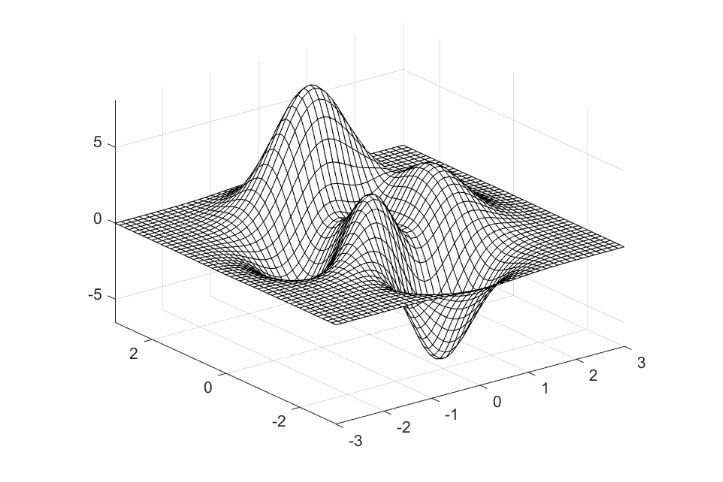
\includegraphics{matlab}

In parallel to MATLAB and R, Python represents the advent of the so-called scripting languages. Scripting languages are programming  languages which offer readability and versatility, along with decoupling from the actual operating system that it is being executed on. System languages, such as C, are designed and used in order to interact directly with the computer hardware, and to constitute data structures from the ground up\cite{ousterhout_scripting_1998}. On the other hand, scripting languages were designed and used in order to connect existing software systems or data sources together, most notably in the early days of shell scripting (such as \lstinline{Bash}, \lstinline{sed} or \lstinline{awk}). Starting with the late 1990s, and the appearance of languages such as Perl\footnote{First version developed in 1987 by Larry Wall} and Python\footnote{First official release in 1991 by Guido Van Rossum}, scripting languages became more widely used by non-programmers who already had data to work with and needed tools to exploit it. In the following decades, the development of additional scientific libraries such as \emph{SciKit}, \emph{NumPy} for mathematics and numerical work or \emph{NLTK} for language processing and social sciences in Python complemented the language's ease of use by providing manipulation of complex scientifc concepts\cite{millman_python_2011}, a phenomenon of user-extension which has also been observed in R and MATLAB's ecosystems\cite{moler_history_2020}.

This steady rise of scientific computing has nonetheless highlighted the apparent lack of quality standards in academic software, and how the lack of value judgments on the software written might impact the reliability of the scientific output. Perhaps the most well-known example of such a lack is the one revealed by the leak of the source code of the Climate Research Unit from the University of East Anglia in 2009\cite{merali_computational_2010}. In the leak, inline comments of the authors, as well as code reviews of external software developers point out to the CRU leak as being a symptom of the state of academic software. As Professor Darrel Ince stated to the UK Parliamentary Committee in February 2010:

\begin{quote}
There is enough evidence for us to regard a lot of scientific software with worry. For example Professor Les Hatton, an international expert in software testing resident in the Universities of Kent and Kingston, carried out an extensive analysis of several million lines of scientific code. He showed that the software had an unacceptably high level of detectable inconsistencies.\cite{committee_disclosure_2010}
\end{quote}

As a response to this realization, the beginning of the 2000s has seen the desire to re-integrate the best practices of software engineering in order to correct scientific software's lack of accuracy\cite{hatton_how_1994}. Indeed, software engineering, as we've seen above, had developed on their own since its establishment as an independent academic discipline and professional field. Such a split, described by Diane Kelly as a "\emph{chasm}"\cite{kelly_software_2007} then had to face the different standards to which commercial software and scientific software are subject to. For instance, commercial software must be extensible and performant, two qualities that do not necessarily translate to an academic setting, in which software might be written within a specific, time-constrained, research project, or in which access to computing resources (i.e. supercomputers) might be less of a problem.

Within Landau et. al's conception of the scientific process as the progression from problem to theory, followed by the establishment of a model, the devising of a method, and then on to implemementation and finally to assessment\cite{landau_survey_2011}, code written as academic software is now involved in the latter two stages of  method and implementation. Within those two stages, software has to abide by the processes and requirements of scientific research. First and foremost, reproducibility is a core requirement of scientific research in general\footnote{This requirement dates back the 1600s with Robert Boyle and the Invisible College in England\cite{leveque_reproducible_2012}} and bugs in a scientific software system can lead to radically different ouptuts given slightly different input data, while concealing the origin of this radical difference. Good academic code, then, is one which defends actively against these, perhaps to the expense of performance and maintainability. This can be addressed by reliable error-handling, regular assertions of the state of the processed data and extensive unit testing\cite{wilson_best_2014}.

Furthermore, a unique aspect of scientific software comes from the lack of clear upfront requirements. Such requirements, in software development, are usually provided ahead of the programming process, and should be as complete as possible. As the activity of scientists is defined by an incomplete understanding of the application domain, requirements tend to emerge as further knowledge is developed and acquired\cite{segal_when_2005}. As a result, efforts have been made to familiarize scientists with software development best practices, so that they can implement quality software by themselves. Along with field-specific textbook\footnote{See \emph{Effective Computation in Physics}\cite{scopatz_effective_2015} or \emph{A Primer for Computational Biology}\cite{oneil_primer_2019} as textbooks covering similar software-oriented material from different academic perspectives.} the most prominent initiative in the field is \emph{Software Carpentry}, a collection of self-learning and teaching resources which aims at implementing software best practices across academia, for scientists and by scientists. Founded by Greg Wilson, the co-editor of \emph{Beautiful Code}, the organization's title refers directly to equivalents in the field of software development\footnote{See 1.1.2 \emph{Features of the field} above fo a discussion of the literature on writing good code for software developers).

We conclude here on a convergence of quality standards of broad academic software towards the quality standards of commercial software development\footnote{See Graphbrain at \url{https://github.com/graphbrain/graphbrain} for such an example. The code's organization and formal features are congruent and on par with commercial software.}.  And yet, this convergence is due to, as we've seen, a past divergence between computation and science, as computer science worked towards asserting and pursuing its own field of research. As a subset of science, computer science nonetheless holds specific standards, taking software not as a means to an end, but as the end itself.

\vspace*{1\baselineskip}

\subsubsection{Computation as an end}

% history
Computer scientists, while scientists as well, are nonetheless focused on computation as a means, rather than as a tool. Computation is the phenomenon which has led to the development of the theoretical framework around it. Originally derived from computability theory, as a branch of formal mathematical logic, computation emerged as an autonomous field from work in mechanical design and configuration (Ada Lovelace and Charles Babbage),  work on circuit and language design (C. S. Pierce, Konrad Zuse and John Von Neumann), work on mathematical foundations (Alan Turing and Alonzo Church), information theory (Claude Shannon), systems theory (Norbert Wiener) and expert systems (John McCarthy and Marvin Minsky)\cite{ifrah_universal_2001}. In the middle of such a constellation ranging from mathematical theory to practical electronics, the first computer science deparment is inaugurated at Purdue University in 1962.

From this multifaceted heritage and academic interdisciplinarity, computer scientists have established the some of the foundations of the field, identifying key areas such as data structures, algorithms and language design as the foundations of the discipline\cite{wirth_algorithms_1976}. Through the process, the tracing of the "roots" of computation remained a constant debate as to whether computer science exists within the realm of mathematics, of engineering or as a part of the natural sciences. The logico-mathematical model of computer science contends that one can do computer science without a computer, solely armed of a pen and a paper, while the engineering approach of computer science tends to put more practical matters, such as architecture, language design and systems programming at the core of the discipline; both being a way to generate and process information as natural phenomenon\cite{tedre_development_2006}.

% a section on how the three (science, eng, maths) separate from one another?
know-of vs. know-how / episteme vs. techne

%re: engineering
In the software engineering debates, the theory and practice vocabulary
had slightly different tones, with terms like “art” and “science” labeling two
different mindsets concerning programming. At the beginning, software engi-
neering suffered from an earlier image of programming as an inherently un-
manageable, unsystematic, and artistic activity. There again, many saw pro-
gramming essentially as an art or craft. Software production itself was torn
from inside in a struggle between elegance and efficiency, between correct-
ness and productivity, between form and function, and between rule-bound
science and intuitive art. In the beginning, when machine time was expen-
sive and every instruction cycle counted, efficiency ruled over elegance, but in
the end elegance prevailed: Among other things, it facilitated good program-
ming habits, improved programmer productivity, worked well with rigorous
processes, made program maintenance less painful, and eased management of
increasingly large programs.

% art of computer programming -> between theory and practice

% art of algorithms and their implementation -> textbook beauty

% an autotelic aesthetic? lisp vs. bad implementations of binary search

\begin{itemize}
    \item PL \& algo implementers (Hoare, data structuring)
    \item textbooks
\end{itemize}

binary search algorithm's implementation is only accurate in  is only found in five out of twenty textbooks Pattis, Richard E. (1988). "Textbook errors in binary searching". SIGCSE Bulletin. 20: 190–194. doi:10.1145/52965.53012.

Naur, P., 1985, “Programming as theory building”, Microprocessing and microprogramming, 15(5): 253–261.

examples of beautiful scientist code:

\begin{itemize}
    \item LISP (full of concepts)
    \item some sort of quicksort -> https://stackoverflow.com/questions/26301/your-favourite-algorithm-and-the-lesson-it-taught-you
    \item fractals?
    \item list of implementations in julia https://github.com/mossr/BeautifulAlgorithms.jl
\end{itemize}

\subsection{Poets - 2000}

\begin{itemize}
    \item history of creative coding
    \item digital art vs. software art
    \item code poets
\end{itemize}


\section{Ideals of beauty - 5000}

\subsection{Introduction to the Methodology - 1000}

Kintsch and Van Dijk

\subsection{Lexical Field in Programmer Discourse -4000}

Positive words (13p)

\begin{itemize}
    \item clean
    \item simple
    \item elegant
    \item transparent/self-explanatory
\end{itemize}

Negative words (2p)

\begin{itemize}
    \item smelly
    \item entangled
\end{itemize}

\section{Types of beauty  - 20p}

Now that we've done some empirical work, we can try to abstract away a bit and then look into how this relates to existing frameworks of aesthetics. 

Now that \emph{we look at proofs, through discourse}, what kind of beauty can we be dealing with?

\subsection{Literary Beauty}

This second approach contrasts with the functional component of the first one, but nonetheless stands in relationship with it. the creative beauty, by defying traditional beauty standards, does help us highlight, through deviance, what the norm is. These texts on "creative beauty" include the classical perl poetry, code poems, IOCC, code poetry contest, etc.

\subsection{Mathematical beauty}

Mostly elegance, could be a good place to work on the distinction between proof and theorem, concept and appearance.

\subsection{Architectural beauty}

This allows a segue into everyday aesthetics and environmental aesthetics

\section{Craft and beauty - 10p}

Now that we've seen how the aesthetic ideals of code borrow from different registers, we need to think about practice, or ways. all of the above can be seen through the prism of craft

\subsection{Functional beauty}

This first approach, by comparing both source and comment at the same time (taking texts which are explicitly described as being beautiful), explicitly highlights the requirements for source code to be beautiful. 

There is also an emerging development in aesthetics of integrating function as a criteria for an aesthetic experience.

\subsection{Embodiment}

also note the place and role of tools (IDEs, teletypes, fast compiling, etc.)

\subsection{Tacit knowledge}

